\documentclass[12pt, a4paper, twocolumn]{article}

% Required Packages
\usepackage{amsmath}
\usepackage{amssymb}
\usepackage{tikz}
\usepackage{pgfplots}
\usepackage{float}
\usepackage{graphicx}
\usepackage[margin=1in]{geometry}
\usepackage{fancyhdr} % Added for copyright footer

% PGFPlots configuration
\pgfplotsset{compat=1.18}

% --- Copyright Footer Configuration ---
\pagestyle{fancy}
\fancyhf{} % Clear all header and footer fields
\renewcommand{\headrulewidth}{0pt} % Remove the default header line
\cfoot{\scriptsize \copyright~Author: Arpit Raj} % Center footer with copyright

% Redefine the 'plain' style so the title page also gets the copyright footer
\fancypagestyle{plain}{
    \fancyhf{}
    \renewcommand{\headrulewidth}{0pt}
    
}
% -------------------------------------

\begin{document}

% --- Numbering Continuation Setup ---
\renewcommand{\thesection}{\Roman{section}} % Changes section numbers to uppercase Roman
\setcounter{section}{25}   % The next \section{} will be 26 (XXVI)
\setcounter{equation}{106} % The next equation will be 107
\setcounter{figure}{25}    % The next \begin{figure} will be 26
\setcounter{table}{12}     % The next \begin{table} will be 13
% ------------------------------------

\maketitle

\section{Implementation of AWGN channel}

\subsection{\textbf{Physical Environment Simulation}}
In a real-world physical environment, vectors do not pass between transmission layers perfectly due to inherent signal degradation and interference. To accurately simulate these physical channel conditions within our deep learning architecture, we insert a specialized neural layer in the middle of our network: the AWGN channel.

\subsection{\textbf{Additive White Gaussian Noise (AWGN)}}
The AWGN channel is mathematically defined by three fundamental properties:
\begin{itemize}
    \item \textbf{A $\rightarrow$ Additive:} The noise is directly added to the signal, rather than being multiplicative.
    \item \textbf{W $\rightarrow$ White:} The noise possesses equal power across the entire frequency spectrum.
    \item \textbf{G $\rightarrow$ Gaussian:} The magnitude of the noise follows a normal (bell curve) representation over time.
\end{itemize}

\subsection{\textbf{SNR Mathematics and Noise Power}}
The ratio of signal power to noise power is defined as the Signal-to-Noise Ratio (SNR).
\begin{equation}
    SNR = \frac{P_{signal}}{P_{noise}}
\end{equation}
From this relationship, the required noise power can be derived as:
\begin{equation}
    P_{noise} = \frac{P_{signal}}{SNR}
\end{equation}
The signal power ($P_{signal}$) is calculated as the expected value of the squared magnitude of the transmitted vector $X$:
\begin{equation}
    P_{signal} = \mathbb{E}\big[|X|^2\big]
\end{equation}
Because SNR is typically provided in decibels (dB), we must convert it to a linear scale before applying it to the tensor:
\begin{equation}
    SNR_{linear} = 10^{\left(\frac{SNR_{dB}}{10}\right)}
\end{equation}

\subsection{\textbf{PyTorch Implementation}}
In PyTorch, the function \texttt{torch.randn} generates a random tensor drawn from a standard normal distribution, $\mathcal{N}(0,1)$. To apply the precise amount of noise corresponding to the target SNR, we scale this base distribution by the standard deviation, which is the square root of the variance (noise power).

The algorithmic implementation follows these steps:
\begin{enumerate}
    \item \textbf{Calculate Noise Power:}
    \begin{equation}
        noise\_power = \frac{signal\_power}{snr\_linear}
    \end{equation}
    \item \textbf{Calculate Standard Deviation:}
    \begin{equation}
        noise\_std\_dev = \texttt{torch.sqrt}(noise\_power)
    \end{equation}
    \item \textbf{Generate Scaled Noise:}
    \begin{equation}
        noise = \texttt{torch.randn\_like}(X) \times noise\_std\_dev
    \end{equation}
    \item \textbf{Calculate Received Signal:}
    \begin{equation}
        received = X + noise
    \end{equation}
\end{enumerate}

\subsection{\textbf{Visualizing Channel Noise Effects}}

To comprehensively understand the destructive capabilities of AWGN, we observe its effects across varying SNR levels on both a continuous analog waveform and a discrete vector point in a 2D space.

% Using figure* so the wide plots span across both columns
\begin{figure*}[htbp]
\centering
\resizebox{\linewidth}{!}{
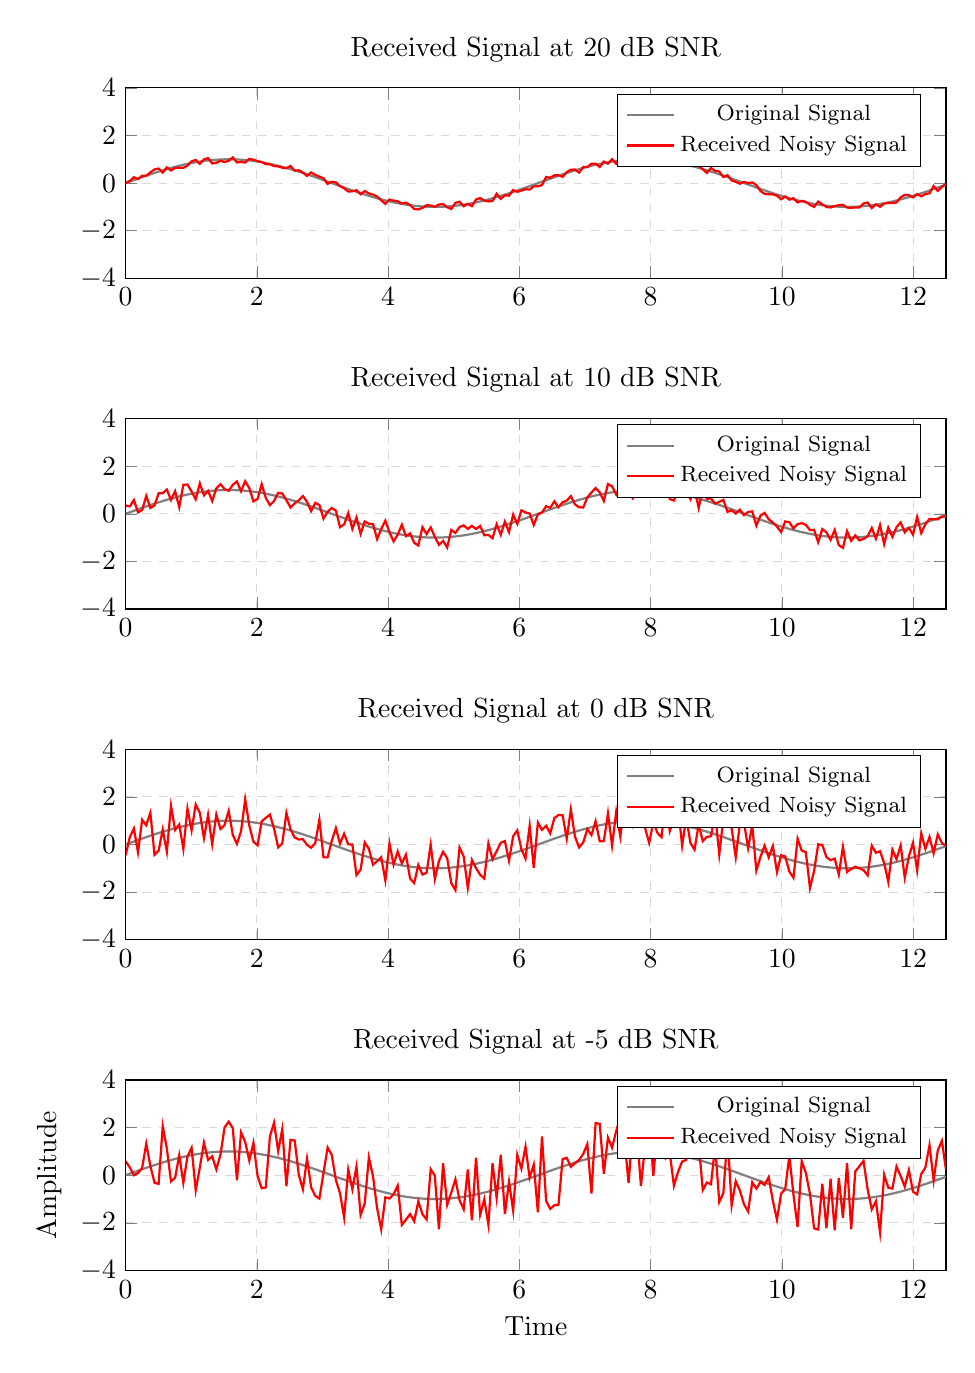
\begin{tikzpicture}
    % Subplot 1: 20dB
    \begin{axis}[
        width=12cm, height=4cm,
        title={Received Signal at 20 dB SNR},
        ymin=-4, ymax=4, xmin=0, xmax=12.5,
        grid=both, grid style={dashed, gray!30},
        legend style={font=\footnotesize},
        legend pos=north east
    ]
        \addplot[thick, gray, domain=0:12.5, samples=200] {sin(deg(x))};
        \addlegendentry{Original Signal}
        \addplot[thick, red, domain=0:12.5, samples=200] {sin(deg(x)) + 0.15*rand};
        \addlegendentry{Received Noisy Signal}
    \end{axis}

    % Subplot 2: 10dB
    \begin{axis}[
        yshift=-4.2cm,
        width=12cm, height=4cm,
        title={Received Signal at 10 dB SNR},
        ymin=-4, ymax=4, xmin=0, xmax=12.5,
        grid=both, grid style={dashed, gray!30},
        legend style={font=\footnotesize},
        legend pos=north east
    ]
        \addplot[thick, gray, domain=0:12.5, samples=200] {sin(deg(x))};
        \addlegendentry{Original Signal}
        \addplot[thick, red, domain=0:12.5, samples=200] {sin(deg(x)) + 0.45*rand};
        \addlegendentry{Received Noisy Signal}
    \end{axis}

    % Subplot 3: 0dB
    \begin{axis}[
        yshift=-8.4cm,
        width=12cm, height=4cm,
        title={Received Signal at 0 dB SNR},
        ymin=-4, ymax=4, xmin=0, xmax=12.5,
        grid=both, grid style={dashed, gray!30},
        legend style={font=\footnotesize},
        legend pos=north east
    ]
        \addplot[thick, gray, domain=0:12.5, samples=200] {sin(deg(x))};
        \addlegendentry{Original Signal}
        \addplot[thick, red, domain=0:12.5, samples=200] {sin(deg(x)) + 1.0*rand};
        \addlegendentry{Received Noisy Signal}
    \end{axis}

    % Subplot 4: -5dB
    \begin{axis}[
        yshift=-12.6cm,
        width=12cm, height=4cm,
        title={Received Signal at -5 dB SNR},
        ymin=-4, ymax=4, xmin=0, xmax=12.5,
        grid=both, grid style={dashed, gray!30},
        xlabel={Time},
        ylabel={Amplitude},
        legend style={font=\footnotesize},
        legend pos=north east
    ]
        \addplot[thick, gray, domain=0:12.5, samples=200] {sin(deg(x))};
        \addlegendentry{Original Signal}
        \addplot[thick, red, domain=0:12.5, samples=200] {sin(deg(x)) + 1.6*rand};
        \addlegendentry{Received Noisy Signal}
    \end{axis}
\end{tikzpicture}
}
\caption{Effect of Additive White Gaussian Noise (AWGN) on a continuous sine wave under degrading Signal-to-Noise Ratio (SNR) conditions.}
\label{fig:awgn_sine}
\end{figure*}

% Using figure* so the side-by-side plots span across both columns
\begin{figure*}[htbp]
\centering

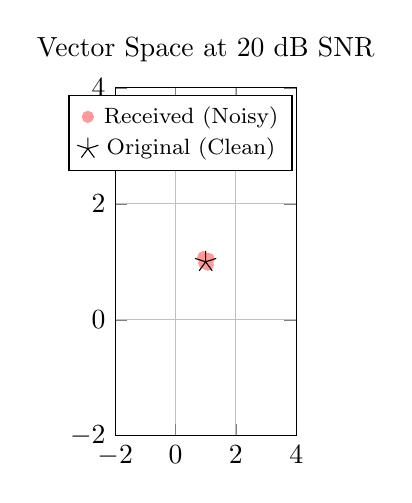
\begin{tikzpicture}
% ---------------- 20 dB ----------------
\begin{axis}[
width=0.32\textwidth,
height=6cm,
title={Vector Space at 20 dB SNR},
xmin=-2,xmax=4,
ymin=-2,ymax=4,
grid=both,
legend style={font=\footnotesize}
]

\addplot[
only marks,
mark=*,
red!40
]
coordinates{
(1.05,1.02)
(0.95,0.98)
(1.10,1.05)
(0.92,1.08)
(1.07,0.95)
};
\addlegendentry{Received (Noisy)}

\addplot[
only marks,
mark=star,
mark size=4pt,
black
]
coordinates{(1,1)};
\addlegendentry{Original (Clean)}

\end{axis}
\end{tikzpicture}%
\hfill%
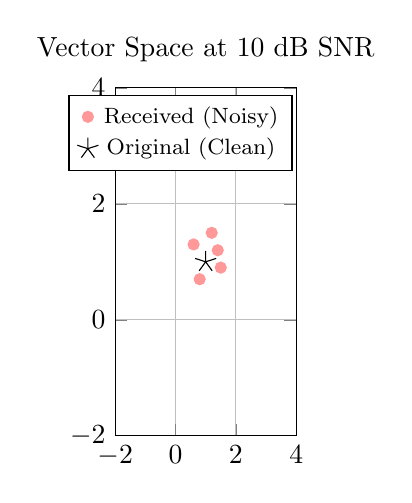
\begin{tikzpicture}
% ---------------- 10 dB ----------------
\begin{axis}[
width=0.32\textwidth,
height=6cm,
title={Vector Space at 10 dB SNR},
xmin=-2,xmax=4,
ymin=-2,ymax=4,
grid=both,
legend style={font=\footnotesize}
]

\addplot[
only marks,
mark=*,
red!40
]
coordinates{
(1.4,1.2)
(0.8,0.7)
(1.2,1.5)
(0.6,1.3)
(1.5,0.9)
};
\addlegendentry{Received (Noisy)}

\addplot[
only marks,
mark=star,
mark size=4pt,
black
]
coordinates{(1,1)};
\addlegendentry{Original (Clean)}

\end{axis}
\end{tikzpicture}%
\hfill%
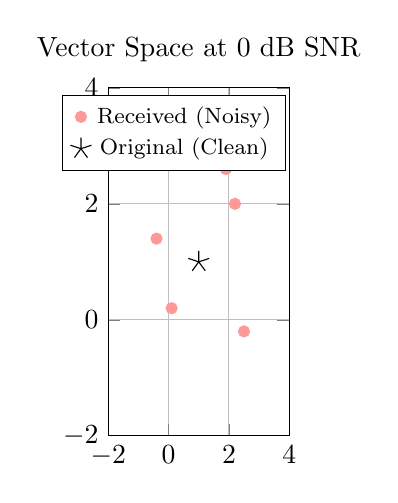
\begin{tikzpicture}
% ---------------- 0 dB ----------------
\begin{axis}[
width=0.32\textwidth,
height=6cm,
title={Vector Space at 0 dB SNR},
xmin=-2,xmax=4,
ymin=-2,ymax=4,
grid=both,
legend style={font=\footnotesize}
]

\addplot[
only marks,
mark=*,
red!40
]
coordinates{
(2.2,2.0)
(0.1,0.2)
(1.9,2.6)
(-0.4,1.4)
(2.5,-0.2)
};
\addlegendentry{Received (Noisy)}

\addplot[
only marks,
mark=star,
mark size=4pt,
black
]
coordinates{(1,1)};
\addlegendentry{Original (Clean)}

\end{axis}
\end{tikzpicture}

\caption{Scattering effect of AWGN on a 2D transmitted vector point $(1,1)$ across decreasing SNR levels.}
\label{fig:awgn_vector}
\end{figure*}

\section{\large \textbf{The LSTM Model}}

\subsection{\textbf{Embedding Dimension vs. Hidden Dimension}}
In the context of the Long Short-Term Memory (LSTM) model, data representations are fundamentally governed by two dimensional spaces:
\begin{itemize}
    \item \textbf{Embedding Dimension:} Controls how words are mathematically represented before transmission. 
    \item \textbf{Hidden Dimension:} Controls the size of the semantic message that is transmitted through the channel.
\end{itemize}

For example, if the embedding dimension is set to 64, all words in the sequence are converted into a 64-dimensional vector representation. The embedding matrix size is given by:
\begin{equation}
    \text{Embedding Matrix} = (\text{Vocab Size} \times \text{Embed Dim})
\end{equation}

Consider a data transmission scenario where:
\begin{itemize}
    \item Batch Size = 32 (representing 32 sentences)
    \item Sequence Length = 10 (representing 10 words per sentence)
    \item Embedding Dimension = 64
\end{itemize}
Before passing through the embedding layer, the tensor shape is $(32, 10)$. After the embedding layer, the shape becomes $(32, 10, 64)$. 

As the tensor processes through the LSTM, the hidden dimension (e.g., 128) maps the current timestep embedding $e_t \in \mathbb{R}^{64}$ into a context space. The network output shape after the LSTM layer becomes $(1, 32, 128)$, successfully converting the input to a context space of 128 dimensions.

\subsection{\textbf{LSTM Architecture and Memory States}}
The LSTM receives two crucial pieces of information at any timestep $t$:
\begin{enumerate}
    \item $e_t$: The current meaning (from the embedding layer).
    \item $h_{t-1}$: The previous sentence context.
\end{enumerate}

The internal architecture relies on two distinct memory pathways. The \textbf{Cell State} ($c_t$) acts as the long-term memory, running through the cell with minimum alteration. Conversely, the \textbf{Hidden State} ($h_t$) acts as the short-term working memory, capturing immediate context, continuously updating, and serving as the direct output of the LSTM cell.

\begin{figure}[h]
\centering
% \resizebox{\columnwidth}{!} forces the tikzpicture to fit within the single column width
\resizebox{\columnwidth}{!}{%
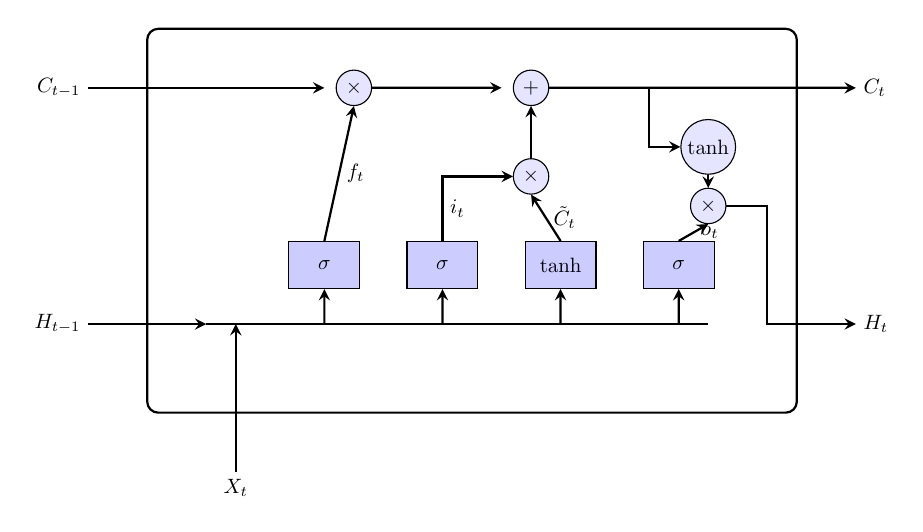
\begin{tikzpicture}[
    >=stealth,
    scale=0.75, transform shape,
    box/.style={draw, rectangle, fill=blue!20, minimum height=0.8cm, minimum width=1.2cm, align=center},
    op/.style={draw, circle, fill=blue!10, inner sep=2pt, minimum size=0.6cm, align=center}
]

    % Main bounding box
    \draw[rounded corners, thick] (-1, -3) rectangle (10, 3.5);

    % Memory line (Cell State)
    \draw[->, thick] (-2, 2.5) node[left] {$C_{t-1}$} -- (2, 2.5);
    \node[op] (mult1) at (2.5, 2.5) {$\times$};
    \draw[->, thick] (mult1.east) -- (5, 2.5);
    \node[op] (add1) at (5.5, 2.5) {$+$};
    \draw[->, thick] (add1.east) -- (11, 2.5) node[right] {$C_t$};

    % Hidden state line
    \draw[->, thick] (-2, -1.5) node[left] {$H_{t-1}$} -- (0, -1.5);
    \draw[thick] (0, -1.5) -- (8.5, -1.5);

    % Input line
    \draw[->, thick] (0.5, -4) node[below] {$X_t$} -- (0.5, -1.5);

    % Forget Gate
    \node[box] (forget) at (2, -0.5) {$\sigma$};
    \draw[->, thick] (2, -1.5) -- (forget.south);
    \draw[->, thick] (forget.north) -- (mult1.south) node[midway, right] {$f_t$};

    % Input Gate & Candidate Memory
    \node[box] (input) at (4, -0.5) {$\sigma$};
    \node[box] (cand) at (6, -0.5) {$\tanh$};
    \draw[->, thick] (4, -1.5) -- (input.south);
    \draw[->, thick] (6, -1.5) -- (cand.south);

    \node[op] (mult2) at (5.5, 1) {$\times$};
    \draw[->, thick] (input.north) |- (mult2.west) node[near start, right] {$i_t$};
    \draw[->, thick] (cand.north) -- (mult2.south) node[midway, right] {$\tilde{C}_t$};
    \draw[->, thick] (mult2.north) -- (add1.south);

    % Output Gate
    \node[box] (output) at (8, -0.5) {$\sigma$};
    \draw[->, thick] (8, -1.5) -- (output.south);
    
    \node[op] (tanh_out) at (8.5, 1.5) {$\tanh$};
    \draw[->, thick] (7.5, 2.5) |- (tanh_out.west);

    \node[op] (mult3) at (8.5, 0.5) {$\times$};
    \draw[->, thick] (output.north) -- (mult3.south) node[midway, right] {$o_t$};
    \draw[->, thick] (tanh_out.south) -- (mult3.north);
    \draw[->, thick] (mult3.east) -| (9.5, -1.5) -- (11, -1.5) node[right] {$H_t$};

\end{tikzpicture}%
}
\caption{Internal computational diagram of an LSTM block detailing gate operations and memory state pathways.}
\label{fig:lstm_cell}
\end{figure}

\subsection{\textbf{Gate Computations and Dimensionality}}
The transition of features from the 64-dimensional embedding to the 128-dimensional hidden space is executed via matrix multiplications within the four neural gates. 

\textbf{1. Forget Gate:}
Determines what information to discard from the cell state.
% Split equations into multiple lines to prevent overflowing into the second column
\begin{align}
    f_t &= \sigma(W_f e_t + U_f h_{t-1} + b_f) \\
    W_f &\in \mathbb{R}^{128 \times 64}, \quad e_t \in \mathbb{R}^{64} \nonumber \\
    &\implies W_f e_t \in \mathbb{R}^{128} \nonumber \\
    U_f &\in \mathbb{R}^{128 \times 128}, \quad h_{t-1} \in \mathbb{R}^{128} \nonumber \\
    &\implies U_f h_{t-1} \in \mathbb{R}^{128} \nonumber
\end{align}
Due to matrix multiplication ($[128 \times 64] \times [64 \times 1] \rightarrow [128 \times 1]$), the 64-dimension embedding is converted to 128 dimensions, establishing $f_t \in \mathbb{R}^{128}$.

\textbf{2. Input Gate and Candidate Memory:}
Determines what new information is stored in the cell state.
\begin{align}
    i_t &= \sigma(W_i e_t + U_i h_{t-1} + b_i) \\
    \tilde{C}_t &= \tanh(W_c e_t + U_c h_{t-1} + b_c)
\end{align}
Following identical dimensional logic, $W_i, W_c \in \mathbb{R}^{128 \times 64}$ and $U_i, U_c \in \mathbb{R}^{128 \times 128}$, yielding $i_t, \tilde{C}_t \in \mathbb{R}^{128}$.

\textbf{3. Output Gate:}
Determines the output based on the filtered cell state.
\begin{align}
    o_t &= \sigma(W_o e_t + U_o h_{t-1} + b_o) \\
    o_t &\in \mathbb{R}^{128} \nonumber
\end{align}

\textbf{4. Memory State Creation:}
The long-term and short-term memory states are updated through element-wise operations ($\odot$):
\begin{align}
    C_t &= f_t \odot C_{t-1} + i_t \odot \tilde{C}_t \\
    h_t &= o_t \odot \tanh(C_t)
\end{align}

\subsection{\textbf{Internal Computation and Parameter Count}}
While conceptually discrete, computational frameworks like PyTorch optimize this by concatenating the inputs at every timestep. The LSTM actually computes $[e_t ; h_{t-1}]$.
\begin{equation}
    \text{Concatenation} \rightarrow 64 + 128 = 192 \text{ dims}
\end{equation}
The framework internally evaluates a combined weight matrix $W [e_t ; h_{t-1}] + b$, where $W \in \mathbb{R}^{128 \times 192}$, effectively mapping $192 \rightarrow 128$.

The total number of parameters required to define the network can be analyzed. For a single gate, the parameter breakdown is:
\begin{equation}
    (128 \times 64) + (128 \times 128) + (128) = 24,704
\end{equation}
This formulation represents:
\begin{itemize}
    \item \textbf{$128 \times 64$}: Evaluates how each of the 64 embedding features affects each of the 128 memory units.
    \item \textbf{$128 \times 128$}: Evaluates how the previous memory influence maps to the current memory.
    \item \textbf{128}: The bias vector ($b$).
\end{itemize}
Since the standard LSTM cell contains exactly 4 independent gates, the total trainable parameters evaluate to:
\begin{equation}
    4 \times 24,704 = 98,816 \text{ parameters}
\end{equation}

\section{\large \textbf{LSTM Architecture (JCC Modelling)}}

\subsection{\textbf{End-to-End System Model}}
The Joint Source-Channel Coding (JCC) model fundamentally operates on an end-to-end framework parameterized by deep learning structures. The overarching mathematical representation of the received and decoded signal $\hat{X}$ is formulated as:
\begin{equation}
    \hat{X} = g_\phi \big( C(f_\theta(X)) \big)
\end{equation}
where:
\begin{itemize}
    \item $f_\theta$ represents the \textbf{semantic encoder}.
    \item $C$ represents the \textbf{AWGN channel}.
    \item $g_\phi$ represents the \textbf{semantic decoder}.
\end{itemize}

\subsection{\textbf{Semantic Encoder}}
The initial stage of the transmission pipeline is the semantic encoder. It maps discrete token IDs into a continuous dense vector space. The embedding vector $e_t$ for a given token sequence $x_t$ is extracted via the embedding function $E$:
\begin{equation}
    e_t = E(x_t)
\end{equation}
The embedding matrix $E$ belongs to the real coordinate space defined by the vocabulary size $V$ and the embedding dimension $d_e$:
\begin{equation}
    E \in \mathbb{R}^{V \times d_e}
\end{equation}

\begin{figure}[htbp]
\centering
\resizebox{\columnwidth}{!}{
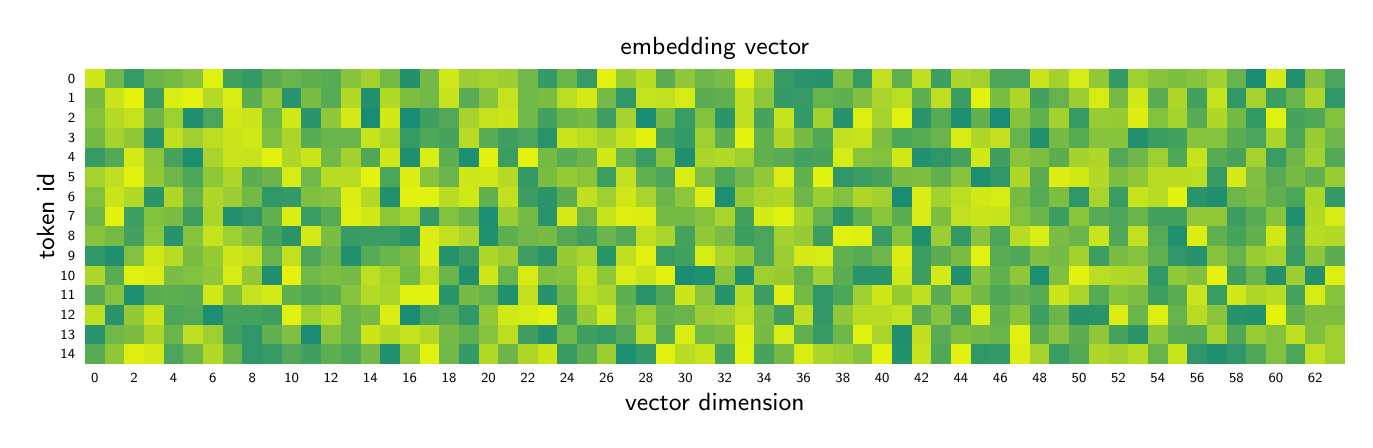
\begin{tikzpicture}[scale=0.25]
    % Draw the heatmap grid simulating the embedding vector
    \foreach \y in {0,...,14} {
        \foreach \x in {0,...,63} {
            \pgfmathsetmacro{\randval}{random(10, 90)}
            \fill[teal!\randval!yellow] (\x, -\y) rectangle (\x+1, -\y-1);
        }
    }
    
    % X-axis labels (vector dimension)
    \foreach \x in {0, 2, ..., 62} {
        \node[below, font=\sffamily\tiny] at (\x+0.5, -15) {\x};
    }
    % Y-axis labels (token id)
    \foreach \y in {0, 1, ..., 14} {
        \node[left, font=\sffamily\tiny] at (0, -\y-0.5) {\y};
    }
    
    % Axis Titles
    \node[below, font=\sffamily\small] at (32, -16) {vector dimension};
    \node[rotate=90, font=\sffamily\small] at (-2, -7.5) {token id};
    \node[above, font=\sffamily\small] at (32, 0) {embedding vector};
\end{tikzpicture}
}
\caption{Heatmap visualization of the dense embedding vector space mapped from discrete token IDs, where $V=15$ and $d_e=64$.}
\label{fig:embedding_vector}
\end{figure}

\subsection{\textbf{LSTM Semantic Compression}}
Following the embedding stage, the sequence of embeddings is processed iteratively by a Long Short-Term Memory (LSTM) network to achieve semantic compression:
\begin{equation}
    (hidden, cell) = \text{self.lstm}(embedded)
\end{equation}
After processing all the words in the sequence, the terminal hidden state $h_T$ contains the concentrated semantic information from the sentence. The encoder returns the tuple $(h_T, C_T)$ to form the latent message.

\subsection{\textbf{Channel Input}}
The latent message components are concatenated to form the final transmitted signal vector $z$:
\begin{equation}
    z = [h_T, C_T]
\end{equation}
The dimensionality of this bottleneck vector $d_z$ is exactly twice the hidden dimension $H$. Given $H = 128$:
\begin{equation}
    d_z = 2H = 2 \times 128 = 256
\end{equation}
This composite vector acts as the transmitted signal over the physical channel.

\begin{figure*}[htbp]
\centering
\begin{tikzpicture}
\begin{axis}[
    width=\textwidth,
    height=4.5cm,
    ybar,
    bar width=2.5pt,
    ymin=-1.1, ymax=1.1,
    xmin=-2, xmax=130,
    ylabel={Activation Value},
    xlabel={z dimension (128-dim)},
    title={semantic bottleneck vector after lstm z},
    grid=y,
    grid style={dashed, gray!30},
    legend pos=north west,
    legend style={font=\footnotesize},
    enlarge x limits=0.02
]
    % Generating synthetic bar data to match the visual of a 128-dim state vector
    \addplot[fill=blue!60, draw=blue!60] expression[domain=0:127, samples=128] {rand};
    \addlegendentry{Hidden State ($h_t$)}
\end{axis}
\end{tikzpicture}
\caption{Activation values of the semantic bottleneck vector representing the mapped LSTM hidden state prior to channel transmission.}
\label{fig:bottleneck_vector}
\end{figure*}

\subsection{\textbf{Noise Modelling}}
During physical transmission, Additive White Gaussian Noise (AWGN) corrupts the latent message. The received noisy representations of the hidden and cell states are:
\begin{align}
    \tilde{h} &= h + n_h \\
    \tilde{c} &= c + n_c
\end{align}
The total signal power $P_s$ is calculated as the mean squared amplitude across $N$ elements:
\begin{equation}
    P_s = \frac{1}{N} \sum_{i=1}^N x_i^2
\end{equation}
Using the defined Signal-to-Noise Ratio in decibels ($SNR_{dB}$):
\begin{equation}
    SNR_{dB} = 10 \log_{10} \left( \frac{P_S}{P_N} \right)
\end{equation}
The required noise power $P_n$ (which equates to the variance $\sigma^2$ of the Gaussian noise) is derived as:
\begin{equation}
    P_n = \frac{P_s}{10^{SNR_{dB}/10}} \quad , \quad \sigma^2 = P_n
\end{equation}

\subsection{\textbf{Semantic Decoder}}
At the receiver side, the semantic decoder reconstructs the intent. During training, the true previous word is fed to the decoder (Teacher Forcing) to calculate the conditional probability:
\begin{equation}
    P(x_t \mid x_{t-1}, h_t)
\end{equation}
The decoder outputs a hidden state $h_t$, which is converted into vocabulary probabilities via a linear transformation:
\begin{equation}
    o_t = W h_t + b \quad \Big( o_t \in \mathbb{R}^V \Big)
\end{equation}
This output $o_t$ is pushed through a Softmax function to generate a valid probability distribution over the vocabulary:
\begin{equation}
    P(w_i) = \frac{e^{o_i}}{\sum_j e^{o_j}}
\end{equation}
The predicted token $\hat{x}_t$ is then selected via an argmax operation:
\begin{equation}
    \hat{x}_t = \arg \max P(w_i)
\end{equation}

\subsection{\textbf{Training Objective}}
The overarching training objective of the system is to minimize the Cross-Entropy Loss $L$ over the sequence of length $T$:
\begin{equation}
    L = - \sum_{t=1}^T \log P(x_t)
\end{equation}
Fundamentally, the encoder and decoder architectures jointly learn to minimize this discrepancy between the original and reconstructed messages:
\begin{equation}
    \min \mathcal{L} \big( g_\phi(C(f_\theta(x))), x \big)
\end{equation}


\end{document}

\end{document}